%% Section 3: Assessment of the W26 analysis -- opening, 3.1 [O III] velocities, 3.2 Halpha velocities
\section{Assessment of the W26 analysis}\label{sec:assess}

Table~\ref{tab:claims} lists the W26 claims that we re-examine and our findings. We begin with the velocities, on which the distance and the two-layer shell model depend; Table~\ref{tab:velocity} lists them by region and dataset.

\subsection{The \texorpdfstring{\Oiii{}}{[O III]} velocity offset is a wavelength-reference artifact}\label{sec:oiii}

W26 states that the LAMOST pipeline corrected the MRS-N spectra for heliocentric motion (W26 Sect.~3.2.3) and quotes a radial-velocity precision of $<1.5$\,\kms{} (W26 Sect.~2.2). W26 Table~4 places \Oiii{} at $+23.8$ to $+26.8$\,\kms{} (P1--P3) but \Nii{} and \Sii{} at $+11.7$ to $+13.3$\,\kms{} (P1--P4). This offset of $\sim$5--15\,\kms{} underlies the 100--150\,pc discrepancy between blue- and red-arm distances, the two-layer shell interpretation (W26 Sect.~4.2) and the \Oiii-only kinematic distance (W26 Sect.~3.3).

The W26 Fig.~3a blue-arm spectrum (Section~\ref{sec:data}) contains the \Ni~$\lambda\lambda$5198, 5200 airglow doublet. On the plotted scale, five sky lines (the doublet and three weaker lines) lie $+1.8\pm0.8$\,\kms{} from their air rest wavelengths \citep{Hanuschik2003,Kramida2024}. An air, heliocentric scale would place them at $-8.3$\,\kms{} (excluded at 12$\sigma$) and a vacuum scale at $+75$ to $+83$\,\kms{} ($\geq87\sigma$; Figure~\ref{fig:oiii}a). The plotted scale is therefore air and topocentric, and lacks the heliocentric correction ($v_{\rm corr}=-8.32$\,\kms{} for the 2024 February~1 exposures; \citealt{Astropy2022}), although the LAMOST pipeline delivers vacuum, heliocentric wavelengths \citep{Luo2015,Ren2021}. W26 Table~4 was measured on the same scale: the W26 Fig.~3b spectra reproduce it to $-1.5\pm2.4$\,\kms, whereas a heliocentric table would lie 10.1\,\kms{} below them (excluded at 4.5$\sigma$).

Measured against the airglow in the same spectrum, \Oiii{} needs no wavelength calibration. In W26 Fig.~3a, \Oiii~$\lambda$5007 lies at $+24.1\pm0.9$\,\kms{} on the plotted scale; removing the $+1.8$\,\kms{} sky offset and a $+0.4$\,\kms{} bias from a solar Fraunhofer blend \citep{Kurucz2005}, and adding $v_{\rm corr}$, gives \vhel{} $=+13.6\pm1.2$\,\kms. The W26 Table~4 \Oiii{} velocities are therefore too high by $10.1\pm1.0$\,\kms, the omitted $v_{\rm corr}$ plus the sky offset. Only W26 Fig.~3a shows the airglow, so the correction is applied in aggregate.

Independent spectra agree (Figure~\ref{fig:oiii}c). DESI DR1 \citep{DESI2026}, whose spectra are vacuum and barycentric \citep{Guy2023}, gives $+14.4\pm1.9$\,\kms{} from 390 on-ridge fibers, and SDSS sky fibers \citep{Abdurrouf2022} give $+9.6\pm2.8$\,\kms. DESI and SDSS alone give $+12.9\pm1.6$\,\kms; with the airglow-referenced value, the weighted mean is \vhel{} $=+13.3\pm1.0$\,\kms{} (\vlsr{} $=+1.2\pm1.0$\,\kms; $\chi^2=2.2$ for 2 degrees of freedom), with a further $\pm1$\,\kms{} estimator systematic. \Oiii{} $-$ \Nii{} becomes $+1.1\pm1.3$\,\kms, against $+13.7\pm2.4$\,\kms{} for W26 P1--P3, and the WIM \Ha{} observed by WHAM \citep{Haffner2003} on the southern filament lies at $+13.8\pm0.8$\,\kms.

The LAMOST pipeline calibration is not the cause. On the W26 plate, LAMOST DR12 \citep{Cui2012} stellar velocities give blue minus red arm $=+0.7\pm0.5$\,\kms{} (76 stars), and both arms agree with Gaia DR3 for six stars \citep{Gaia2023,Katz2023}. The simplest explanation is that the blue arm was re-referenced to air sky-line wavelengths after the pipeline, which removed the heliocentric correction; \citet{Ren2021} and \citet{Wu2022} document sky-line recalibration of the red arm only. The correction does not depend on this mechanism.

The \Oiii--red-line offset is therefore not a property of the nebula, and the quoted $<1.5$\,\kms{} precision does not apply to the published blue-arm velocities. The two-layer shell and inhomogeneous-bubble scenarios and the blue/red distance discrepancy are not supported, and the \Oiii{} kinematic distances rest on \vlsr{} $=+11$ to $+16$\,\kms{} instead of the corrected $+1$ to $+5$\,\kms{} (Section~\ref{sec:distance}). Velocity does not separate the \Oiii{} filament from the WIM.

\begin{figure*}
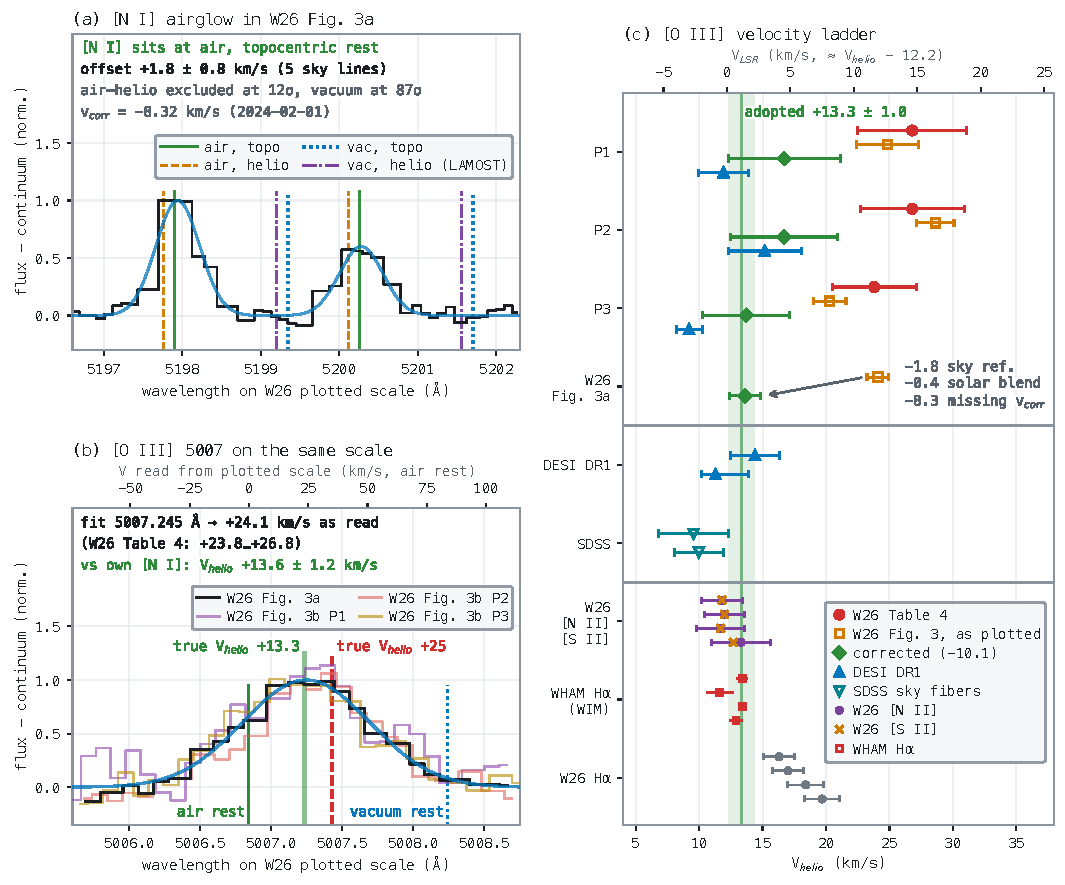
\includegraphics[width=\textwidth]{figures/dispute_oiii_fig3.pdf}
\caption{Wavelength frame of the blue-arm spectra re-extracted from W26 \citep{Wu2026} Fig.~3, and the resulting \Oiii{} velocities. (a) \Ni~$\lambda\lambda$5198, 5200 airglow in W26 Fig.~3a with a two-Gaussian fit. Lines: doublet positions on air or vacuum, topocentric or heliocentric scales. (b) \Oiii~$\lambda$5007 in W26 Fig.~3a (with Gaussian fit) and W26 Fig.~3b (P1--P3), normalized. Lines: air and vacuum rest wavelengths, and plotted positions for true \vhel{} $=+13.3$ and $+25$\,\kms; top axis: plotted-scale velocity. (c) \vhel{} (top axis: \vlsr{} $\approx$ \vhel{} $-\,12.2$\,\kms). P1--P3: W26 Table~4, W26 Fig.~3b as plotted, W26 Table~4 minus 10.1\,\kms, and DESI DR1 within $0.5\arcdeg$. Other rows: W26 Fig.~3a as plotted and referenced to its airglow; DESI \citep{DESI2026} and SDSS \citep{Abdurrouf2022} estimates (Table~\ref{tab:velocity}, note a); and, for P1--P4, W26 \Nii, \Sii{} and \Ha{} and nearest-beam WHAM \Ha{} (\citealt{Haffner2003}; Table~\ref{tab:velocity}). Band: adopted value.\label{fig:oiii}}
\end{figure*}

\subsection{The \texorpdfstring{\Ha{}}{H-alpha} velocities are red-biased}\label{sec:halpha}

W26 Table~4 gives \Ha{} velocities of $+16.3$ to $+19.7$\,\kms{} for P1--P4, W26 Fig.~5 maps the \Ha{} \vlsr, and W26 Sect.~3.2.3 prefers \Ha{} in P4 for its smaller uncertainty. In every region \Ha{} is redder than \Nii{} and \Sii{} from the same red-arm spectra: weighted over P1--P4, \Ha{} $-$ \Nii{} $=+5.5\pm1.1$\,\kms{} (4.9$\sigma$), whereas \Nii{} $-$ \Sii{} $=+0.1\pm1.4$\,\kms{} (Figure~\ref{fig:halpha}d). Relative to the nearest WHAM beams, \Ha{} $-$ WHAM $=+4.8\pm0.7$\,\kms{} but \Nii{} $-$ WHAM $=-0.8\pm1.0$\,\kms. The offset is equally large in the nebula-free P4.

A frame error would shift \Nii{} and \Sii{} as well, and a wavelength-scale error would be largest for \Sii, the line farthest from the red-arm sky-line calibration range of 6287--6553\,\AA{} (air; \citealt{Ren2021,Wu2022}); yet \Sii{} agrees with \Nii{} and WHAM. An erroneous \Ha{} rest wavelength cannot be excluded, but it would have to be $6564.49\pm0.02$\,\AA, below every \ion{H}{1} $n=2$--3 component listed by \citet{Kramida2024}, and would also be an artifact.

Geocoronal \Ha{} offers a plausible mechanism. On 2024 February~1 it lay 22--25\,\kms{} from the WIM line, within one instrumental FWHM (34.5\,\kms; \citealt{Zhang2021}). The MRS-N pipeline subtracts a sky template whose intensity is predicted from the solar altitude \citep{Zhang2021,Wu2022}; on this plate the subtracted sky is 0.86--1.27 times the published nebular \Ha. In our forward model, only over-subtraction shifts the fitted centroid redward by more than 0.4\,\kms{} (Figure~\ref{fig:halpha}a,b). A joint fit to the W26 \Ha{} offsets and widths, with the WHAM width as the true width, requires 30\% (24--33\%) over-subtraction (Figure~\ref{fig:halpha}b,c) and reproduces about three-quarters of the offset, or about one-half with the template fixed at the pipeline position. Fitting the offsets alone requires 47\% but predicts intrinsic widths of 13--23\,\kms, against 31.0--32.4\,\kms{} in W26 Table~2. These are model results, not fits to spectra: the spectra and that night's geocoronal intensity are not available.

The bias itself does not depend on the model. The \Ha{} velocities of W26 Table~4 and W26 Fig.~5 carry a systematic error of $+4.5$ to $+6.7$\,\kms{} that the quoted 1.2--1.4\,\kms{} uncertainties do not include, and the \Ha-based kinematic distances inherit it. These values need confirmation, for example by a re-reduction with the geocoronal intensity left free or the \Ha{} centroid tied to \Nii. The W26 inference of a DIG contribution to the red-arm lines (W26 Sect.~4.2) is unaffected, because the bias is the same on and off the nebula.

\begin{figure*}
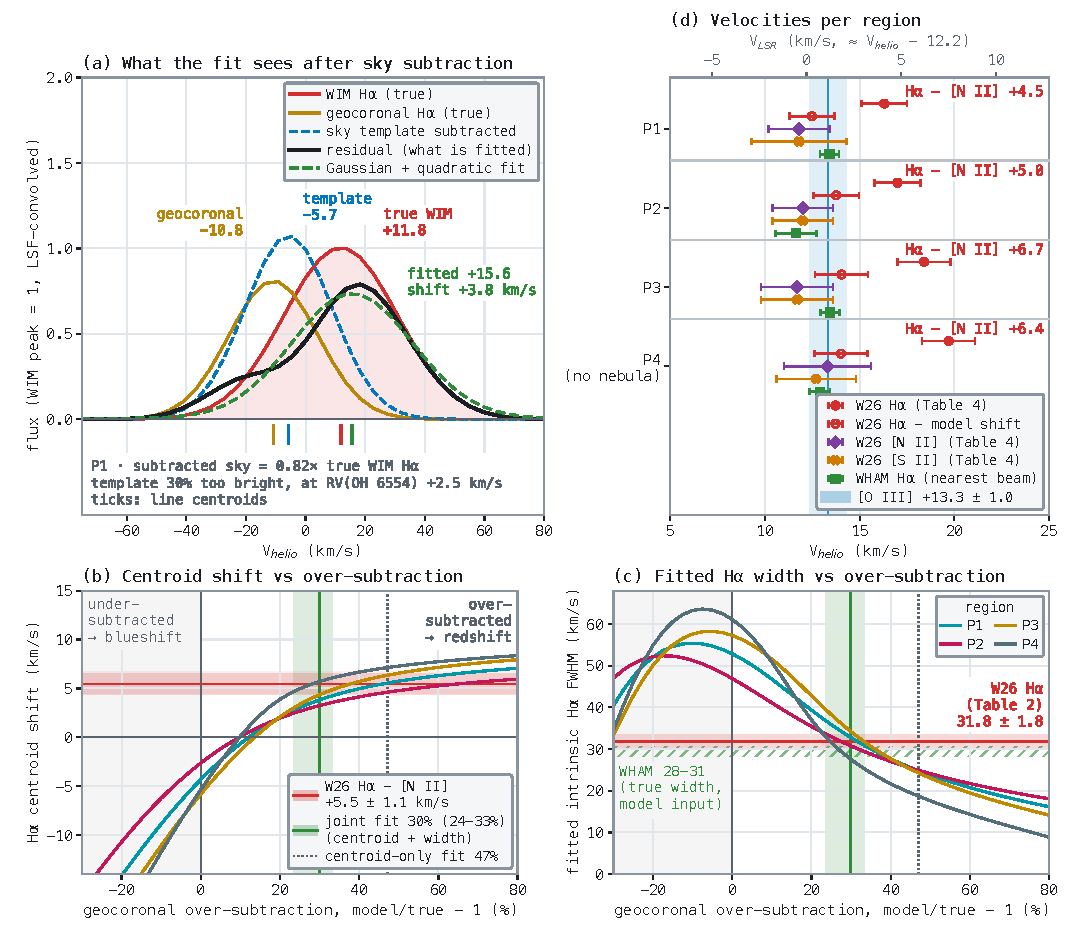
\includegraphics[width=\textwidth]{figures/dispute_halpha_fig4.pdf}
\caption{Forward model of geocoronal \Ha{} over-subtraction by the MRS-N sky template \citep{Zhang2021}, fitted to published W26 values \citep{Wu2026} and not to spectra, and red-line velocities by region. Profiles in (a) are convolved with the instrumental line-spread function (LSF). (a) P1 at the joint centroid-and-width fit: WIM \Ha{} (W26 \Nii{} velocity; WHAM width, \citealt{Haffner2003}), geocoronal \Ha, subtracted template (30\% too bright, $+2.5$\,\kms{} from the OH $\lambda$6554 velocity), residual and its Gaussian-plus-quadratic fit; ticks: centroids. (b) Fitted centroid shift versus over-subtraction for P1--P4 at the joint-fit template position. Horizontal bands: W26 \Ha{} $-$ \Nii{} (weighted mean; P1--P4 range); vertical band: joint fit; dotted line: centroid-only fit. (c) As (b) for the fitted intrinsic \Ha{} FWHM; band: W26 Table~2 mean; hatched: WHAM widths. (d) \vhel{} of \Ha, \Nii{} and \Sii{} (W26 Table~4), \Ha{} minus the model shift, and nearest-beam WHAM \Ha; labels: \Ha{} $-$ \Nii; band: adopted \Oiii{} velocity; top axis: \vlsr{} $\approx$ \vhel{} $-\,12.2$\,\kms.\label{fig:halpha}}
\end{figure*}

\begin{deluxetable*}{lccccc}
\tablecaption{Heliocentric velocities by region and dataset (km\,s$^{-1}$)\label{tab:velocity}}
\tablehead{
\colhead{Dataset, line} & \colhead{P1} & \colhead{P2} & \colhead{P3} & \colhead{P4 (no nebula)} & \colhead{Aggregate\tablenotemark{a}}
}
\startdata
W26 Table~4, \Oiii & $+26.8\pm4.3$ & $+26.8\pm4.1$ & $+23.8\pm3.3$ & \nodata & $+25.5\pm2.2$ \\
\Oiii{} corrected ($-10.1\pm1.0$) & $+16.7\pm4.4$ & $+16.7\pm4.2$ & $+13.7\pm3.5$ & \nodata & $+15.4\pm2.3$ \\
\Oiii{} vs.\ W26 \Ni{} airglow (W26 Fig.~3a) & \nodata & \nodata & \nodata & \nodata & $+13.6\pm1.2$ \\
DESI DR1, \Oiii\tablenotemark{b} & $+11.9\pm1.9$ (61) & $+15.2\pm2.9$ (9) & $+9.2\pm1.0$ (128) & \nodata & $+14.4\pm1.9$ \\
SDSS sky fibers, \Oiii & \nodata & \nodata & \nodata & \nodata & $+9.6\pm2.8$ \\
Adopted \Oiii & \nodata & \nodata & \nodata & \nodata & $+13.3\pm1.0$ \\
W26 Table~4, \Nii & $+11.8\pm1.6$ & $+12.0\pm1.6$ & $+11.7\pm1.9$ & $+13.3\pm2.3$ & $+12.2\pm0.9$ \\
W26 Table~4, \Sii & $+11.8\pm2.5$ & $+12.0\pm1.6$ & $+11.7\pm1.9$ & $+12.7\pm2.1$ & \nodata \\
WHAM, \Ha\tablenotemark{c} & $+13.4\pm0.4$ & $+11.6\pm1.1$ & $+13.4\pm0.3$ & $+12.9\pm0.5$ & $+13.8\pm0.8$ \\
W26 Table~4, \Ha & $+16.3\pm1.2$ & $+17.0\pm1.2$ & $+18.4\pm1.4$ & $+19.7\pm1.4$ & \nodata \\
\enddata
\tablecomments{W26 values are as published. \vlsr{} $=$ \vhel{} $+\,\Delta V$, with $\Delta V=-12.10$, $-11.87$, $-12.58$ and $-12.38$\,\kms{} for P1--P4 and $-12.2$\,\kms{} (mean southern value) for the aggregate column (Section~\ref{sec:data}).}
\tablenotetext{a}{W26 and corrected \Oiii: P1--P3 weighted mean. \Ni{} airglow: one spectrum of unstated position. DESI: on-ridge stack of 390 fibers, including a $\pm1.5$\,\kms{} zero-point uncertainty; a joint fit to both \Oiii{} lines gives $+11.3$ (16--84\%: 10.2--13.9). SDSS: ON$-$OFF stack of all strands; an independent reduction gives $+12.3\pm2.5$ (all strands) and $+10.0\pm1.8\pm0.8$ (Dec $<20\arcdeg$). Adopted: weighted mean of the airglow-referenced, DESI and SDSS values. \Nii: unweighted mean of P1--P4. WHAM: mean and beam-to-beam scatter of six beams on the southern filament, converted beam by beam (\vlsr{} $=+1.3$\,\kms{} as observed; mean $\Delta V=-12.5$\,\kms).}
\tablenotetext{b}{Weighted mean of positive-residual fibers with S/N $>4$ within $0.5\arcdeg$ (number in parentheses), without the zero-point uncertainty (Appendix~\ref{sec:appendix-desi}). P2 (Dec $+17.7\arcdeg$) lies at the southern edge of the zone (Dec 17.6--21$\arcdeg$) where DESI, but not SDSS, gives $+17$ to $+23$\,\kms{} (Section~\ref{sec:spectrum}).}
\tablenotetext{c}{Main component of the nearest $1\arcdeg$ beam ($0.27$--$0.48\arcdeg$ away); the uncertainty is the beam-to-beam scatter within $1\arcdeg$.}
\end{deluxetable*}
